\chapter{Methodology}\label{cap:metodology}
The methodology section explores an approach to software development, starting with the definition of requirements, moving on to the method of data reception, and the selection of technologies. The development process incorporates the creation of user stories, organized on a Kanban board for task management, and the configuration of repositories. Documentation and regular meetings that track progress are a constant in all phases to ensure that the project is proceeding as expected.

\section{Development Methodology}
In the field of software development methodologies, the article \cite{shankarmani2012agile} provides valuable insights into the iterative nature of agile processes. The article emphasizes the importance of iterative cycles that deliver tangible and usable results after each iteration. Furthermore, it discusses the role of customer checkpoint reviews for quality assurance at the end of each iteration, ensuring that the work aligns with predefined quality standards. The article also highlights the importance of post-release reviews that generate feedback for improvement plans, which is of utmost importance for the process.

These agile practices are particularly relevant to the current project. Given the focus on real-time data analysis and alert systems, the iterative approach and feedback mechanisms discussed in Shankarmani's article can be instrumental. Specifically, iterative cycles can facilitate incremental development and refinement of system modules to better meet needs according to received feedback. Furthermore, the feedback generated by post-version reviews can be invaluable for improving the overall quality and performance of the system, especially when the software is put into production.

Thus, the agile methodologies discussed in the article can serve as a guiding framework for managing the evolutionary process of the system over time, ensuring its adaptability and adequate responsiveness to the context and needs of the company.

\section[Requirements Definition]{Requirements Definition}\label{sec:req}The precise definition of requirements is crucial to ensure that the developed system meets the project's needs and objectives in an agile way \cite{asghar2016role}. The requirements of this project were classified into functional and non-functional categories, to ensure a complete understanding of what is expected from the system.

\subsection[Functional Requirements]{Functional Requirements}
Functional requirements play a fundamental role in system development, defining the functions that a system or software component should be able to perform. Essentially, they provide a description of the interactions the system will have with its users or other systems, specifying the services the system should provide.

To ensure effectiveness, functional requirements must be clearly defined, unambiguous, and measurable, traceable, complete, and consistent. Moreover, they should be defined considering the needs and objectives of the project, ensuring that the developed system is not only technically sound but also useful and relevant to its end users.

Within the context of the developed system, the functional requirements of the system and their description are listed below, to clearly state, functionally, what the system should do.

\subsubsection{FR1 - The system must allow a user to securely access the system with an email and password}Given that the system is for viewing the operational data of a stamping industry, the information provided should only be accessed by previously authorized users.

\subsubsection{FR2 - The system must allow a user to view their personal information that is stored in the system}
Each user who has access to the system will have some of their personal data registered in it, such as email, position, and type of access. Therefore, each user should have access to their personal information that is saved in the system.

\subsubsection{FR3 - The system must display in real time the values read by the sensors in each of the machines}Upon receiving the data sent by the sensors, the system should display on screen the read values, separated by sensor type and machine.

\subsubsection{FR4 - The system must store an ideal maximum value for each type of sensor used}
Each sensor should have an ideal maximum value for operation. It will serve as a parameter to understand whether the value read by the sensor indicates good or poor machine performance.

\subsubsection{FR5 - The system must identify whenever a value read by the sensor is not below the ideal value}
This requirement refers to the system's ability to automatically detect every time the sensor indicates a value that is not below the pre-defined limit. That is, if the ideal value is X, and the sensor reads a value greater than or equal to X, the system will recognize this situation.

\subsubsection{FR6 - The system must always register when a value read by the sensor is not in accordance with the ideal value}
This requirement implies that the system must keep a record of all times when the value detected by the sensor is not below the stored ideal value.

\subsubsection{FR7 - The system must display on screen when a value read by the sensor is not below the ideal}
Whenever the sensor detects a value below the ideal standard, the system should display an alert on the interface so that it is always visible to the user.

\subsubsection{FR8 - The system must display in notification format the records of non-operation below the ideal value}This requirement establishes that the system should present to users in the form of notifications when the sensor reads a value above the ideal, to enable users to be informed, even if later, whenever an alert is identified.

\subsubsection{FR9 - The system should allow the user to mark a notification as read, so that it does not appear again}
After being notified, users should have the ability to mark this notification as "read", ensuring that the same information does not continue to be displayed repeatedly.

\subsubsection{FR10 - The system should display graphs showing the values read by the sensors on previous days in an aggregated manner, separating by machines}This requirement ensures that users can view, through graphical representations, the readings of sensors from previous days in an aggregated manner. These graphs should be categorized by machine, providing a detailed analysis of the performance of each piece of equipment over time.

\subsubsection{FR11 - The system must display in the graphs a statistical analysis of the machines' operation, along with the maximum ideal operating value}
The graphs should provide a statistical analysis, showing the statistical indicators of the aggregated data average, median, 75th percentile, and average removing outliers. Along with this, the graph will also show the ideal value, serving as a reference for evaluating performance.

\subsubsection{FR12 - The system must allow filtering the information displayed on screen by machines}
Users should have the flexibility to select and view specific information for certain machines, allowing them to focus on specific equipment as needed.

\subsubsection{FR13 - The system must allow filtering the charts displayed on screen by date}
The system should offer the ability for users to filter graphic displays by specific dates, allowing for detailed temporal analyses and comparisons between different periods.

\subsubsection{FR14 - The system must display the machine stoppage charts in a way that exemplifies the display of this data}The system should display machine stops according to the data passed by the spreadsheets with the data. In this way, it can be exemplified how the machine stop information would look if the system received this information.

\subsection[Non-Functional Requirements]{Non-Functional Requirements}\label{ssubec:reqNfuctional}
Non-functional requirements are specifications that determine the performance characteristics, usability, reliability, and other properties that the system must possess, rather than specific behaviors it should demonstrate. While functional requirements describe what a system should do, non-functional requirements specify how the system should perform these functions.

These requirements are crucial to ensure user satisfaction and the operational effectiveness of the system, playing a fundamental role in the quality and overall operation of a software product.

Non-functional requirements can be of various types, such as usability, performance, security, availability, maintenance, and reliability. Within the context of the developed system, the non-functional requirements of the system and their description are listed below, to make clear what was taken into account when developing each of the system's functionalities.

\subsubsection{NFR1 - Availability}The system must have automatic reconnection mechanisms that activate when connection problems or data reception from sensors are detected, thus ensuring the continuity in data reception.

\subsubsection{NFR2 - Access Security}
The system must implement access controls so that only authorized employees have permission to access data and functionalities relevant to their role.

\subsubsection{NFR3 - Network Security}
To ensure the security of data transmission, the connection to the system must be established using the \gls{HTTPS} protocol, which incorporates the \gls{TLS} security layer, thus protecting the data against interceptions and alterations.

\subsubsection{NFR4 - Real-time Transmission}
The system must process and transmit the data sent by the sensors in a streaming-based architecture. The delay between the sensor sending the data and its visualization by the end user should be less than three seconds.

\subsubsection{NFR5 - Modularity}
The system's architecture should be modular, allowing for the integration and addition of new components or functionalities in an efficient manner without compromising the operation of the existing parts.

\subsubsection{NFR6 - Maintainability}
Prioritizing longevity and ease of maintenance, the system should be developed following good programming practices and system modularization. This will facilitate future modifications, expansions, and the correction of any potential problems.

\subsubsection{NFR7 - Scalability of sensors and machines}
The system design must be able to handle an increasing volume of sensors and machines, ensuring that there is no performance degradation or failures when the demand for resources increases.

\subsubsection{NFR8 - Portability}
The system must ensure compatibility with the main web browsers available on the market. In addition, the user interface should adapt well on larger screens such as televisions, allowing the dashboard to be clearly viewed in different factory environments.

\subsubsection{NFR9 - Usability}The system interface and its components should be designed considering fundamental principles of interaction design, ensuring that users can understand and interact with the system in an intuitive and efficient manner.

\section[Data Collection and Storage Method]{Data Collection and Storage Method}

Within the project context, the way sensor data is collected and stored greatly influences the system's operation, as it is from them that the entire system is structured. Thus, a protocol developed in another project within the same context of the \texttt{Attract Project} was used as a basis, which transmits all the necessary information for the context of this project. Within the system in question, the responsibility of implementing the decoder for the given protocol was assigned.

The protocol format is structured to represent the information pertinent to the machine, the type of communication, the sensor, and the meaning of the transmitted data, following the format below:

\subsubsection{Machine ID (2 bytes)}

The \textit{Machine ID} field is responsible for identifying the machine in question and is divided into two subfields:

\begin{itemize}
    \item \textbf{High (higher order bytes)}: Represents the type of machine. Possible values include: press, lathe, robot, conveyor, among others.
    \item \textbf{Low (lower order bytes)}: Identifies the machine number.
\end{itemize}

\subsubsection{Type (1 byte)}

The \textit{Type} field indicates the type of message and can assume the following values:
\begin{enumerate}
    \item Publish
    \item Request to publish
\end{enumerate}

\subsubsection{Sensor ID (2 bytes)}

The \textit{Sensor ID} field provides details about the sensor that is transmitting the data:

\begin{itemize}
    \item \textbf{High (higher order bytes)}: Represents the physical quantity being measured, such as temperature, speed, pressure, force, among others.
    \item \textbf{Low (lower order bytes)}: Indicates the sensor number.
\end{itemize}\subsubsection{Meaning of Data (2 bytes)}

The \textit{Meaning of Data} field provides information about the type and meaning of the data:

\begin{itemize}
    \item \textbf{High (higher order bytes)}: Data type:
    \begin{enumerate}
        \item Not defined
        \item Normal
        \item Raw data
        \item Alarm
    \end{enumerate}
    \item \textbf{Low (lower order bytes)}: Meaning of the data, which varies according to the equipment. Examples include:
    \begin{itemize}
        \item Oil critical temperature
        \item Check oil temperature
        \item Oil pressure
\end{itemize}
\end{itemize}

\subsubsection{Length (2 bytes)}

The \textit{Length} field indicates the number of subsequent bytes in the package.

\subsubsection{Data}

This field represents the data transmitted by the sensor. The exact specification of what the data represents should be defined and standardized, as indicated by the notation (*).


\section[Software development process]{Software development process}
With a clear definition of the system requirements and how the data read by the sensors are transmitted, the process of how the project would be developed was defined. This development process involves defining user stories, organizing activities, organizing documentation, setting up repositories on GitHub, and holding regular meetings with the supervising professor and the company to discuss progress.

\subsection{User Stories}
In agile software development, one of the most user-centered approaches to understanding system features and requirements is the use of \textit{user stories}. These are short, simple, and informal descriptions from the perspective of an end user, capturing what they need or want to do in the software \cite{lucassen2015forging}.

The typical structure of a user story is: "As a [type of user], I want [an action] so that [a benefit/outcome]". This structure helps to keep the focus on the user's needs and desires, rather than prematurely diving into technical solutions or implementation details.

In addition to being a communication tool between developers and stakeholders, user stories facilitate task prioritization, assist in creating acceptance criteria, and provide a basis for interactive discussions during review and planning meetings.

In short, user stories serve as an effective means of translating complex requirements into manageable, user-centered tasks, ensuring that the final product meets the expectations and needs of its users.

With this definition of user stories, the following items were defined that translate the requirements into tasks for the project development:

\begin{enumerate}
    \item As a user, I must be able to log in with my credentials to use the system.
    \item As a user, I should be able to view my personal information on a profile page to manage the data the system holds about me.
    \item As a user, I should be able to view in real-time values of the machines to detect relevant variations in operation more quickly.
    \item As a user, I should be able to view the historical values of the sensors aggregated in charts of the machines to monitor the status over time.
    \item As a user, I should be able to filter the dashboard information by machine and by date to view data according to my needs.
    \item As a user, I should be alerted when a sensor reads a value that exceeds the ideal parameter so I can take necessary actions as quickly as possible.
    \item As a user, I should be able to view system notifications to be alerted about machine operation alerts.
    \item As a user, I should be able to view the machine downtime records for a better and more organized view of the recorded machine downtimes.
    \item As a user, I should be able to view the system information (dashboards) on different screen sizes so that I can display the information in different contexts.
\end{enumerate}

Each of these user stories was further detailed in the task organization, including a more complete description, possible business rules, which requirements, functional and non-functional, it refers to, and also acceptance criteria. The organization of activities is detailed in section \ref{sec:taskOrganization}.


\subsection{Task Organization}\label{sec:taskOrganization}
The Kanban method, originating from the Toyota production system, has become a popular and effective tool for managing and organizing workflows. The word "Kanban" is of Japanese origin and can be translated as "visual card" or "signage". In the context of project management, Kanban refers to a visual management system that highlights the workflow and tasks at different stages of the process. The essence of Kanban is to visualize the entire workflow, from tasks that have not yet been started to those that have been completed. This visualization allows the identification of bottlenecks and inefficiencies, thus optimizing the process \cite{ghani2015agile}. For the organization of the activities of this project, the Kanban method was adopted as a strategy to ensure an efficient and systematic progression of work.

For the implementation of the Kanban method, Notion was chosen as the tool. The choice of this software is due to its flexibility and customization capacity, allowing the creation of a Kanban board that specifically adapts to the project's needs \cite{notionProjectManagement}. In addition, Notion offers an intuitive interface for building documentation, which is further detailed in section \ref{sec:documentation}.

The Kanban board was structured into five columns, each representing a distinct stage in the workflow:

\begin{itemize}
    \item \textbf{Backlog:} This column contains all identified tasks and activities that have not yet been started. It is a repository of everything that needs to be done, but does not yet have a defined start date.
    \item \textbf{To Do:} The tasks in this column are ready to be started. They have been taken from the Backlog, detailed, and have priority to be started soon.
    \item \textbf{Stopped:} Here are the tasks that have been started, but for some reason had to be interrupted, from changes in priority, the need for some validation, or technical limitation.
    \item \textbf{In Progress:} This column contains the tasks that are currently underway. The move to this column indicates that work is actively being done on the task.
    \item \textbf{Done:} As soon as the development of a task is completed, it is marked as completed, and therefore, moved to this column. It represents the success in completing the activity, and serves as a record of all completed items.
\end{itemize}

The structuring of these columns provides a clear view of the status of each activity and helps to quickly identify where the bottlenecks are, facilitating decision-making and task prioritization.

\begin{figure}[htbp]
	\centering
	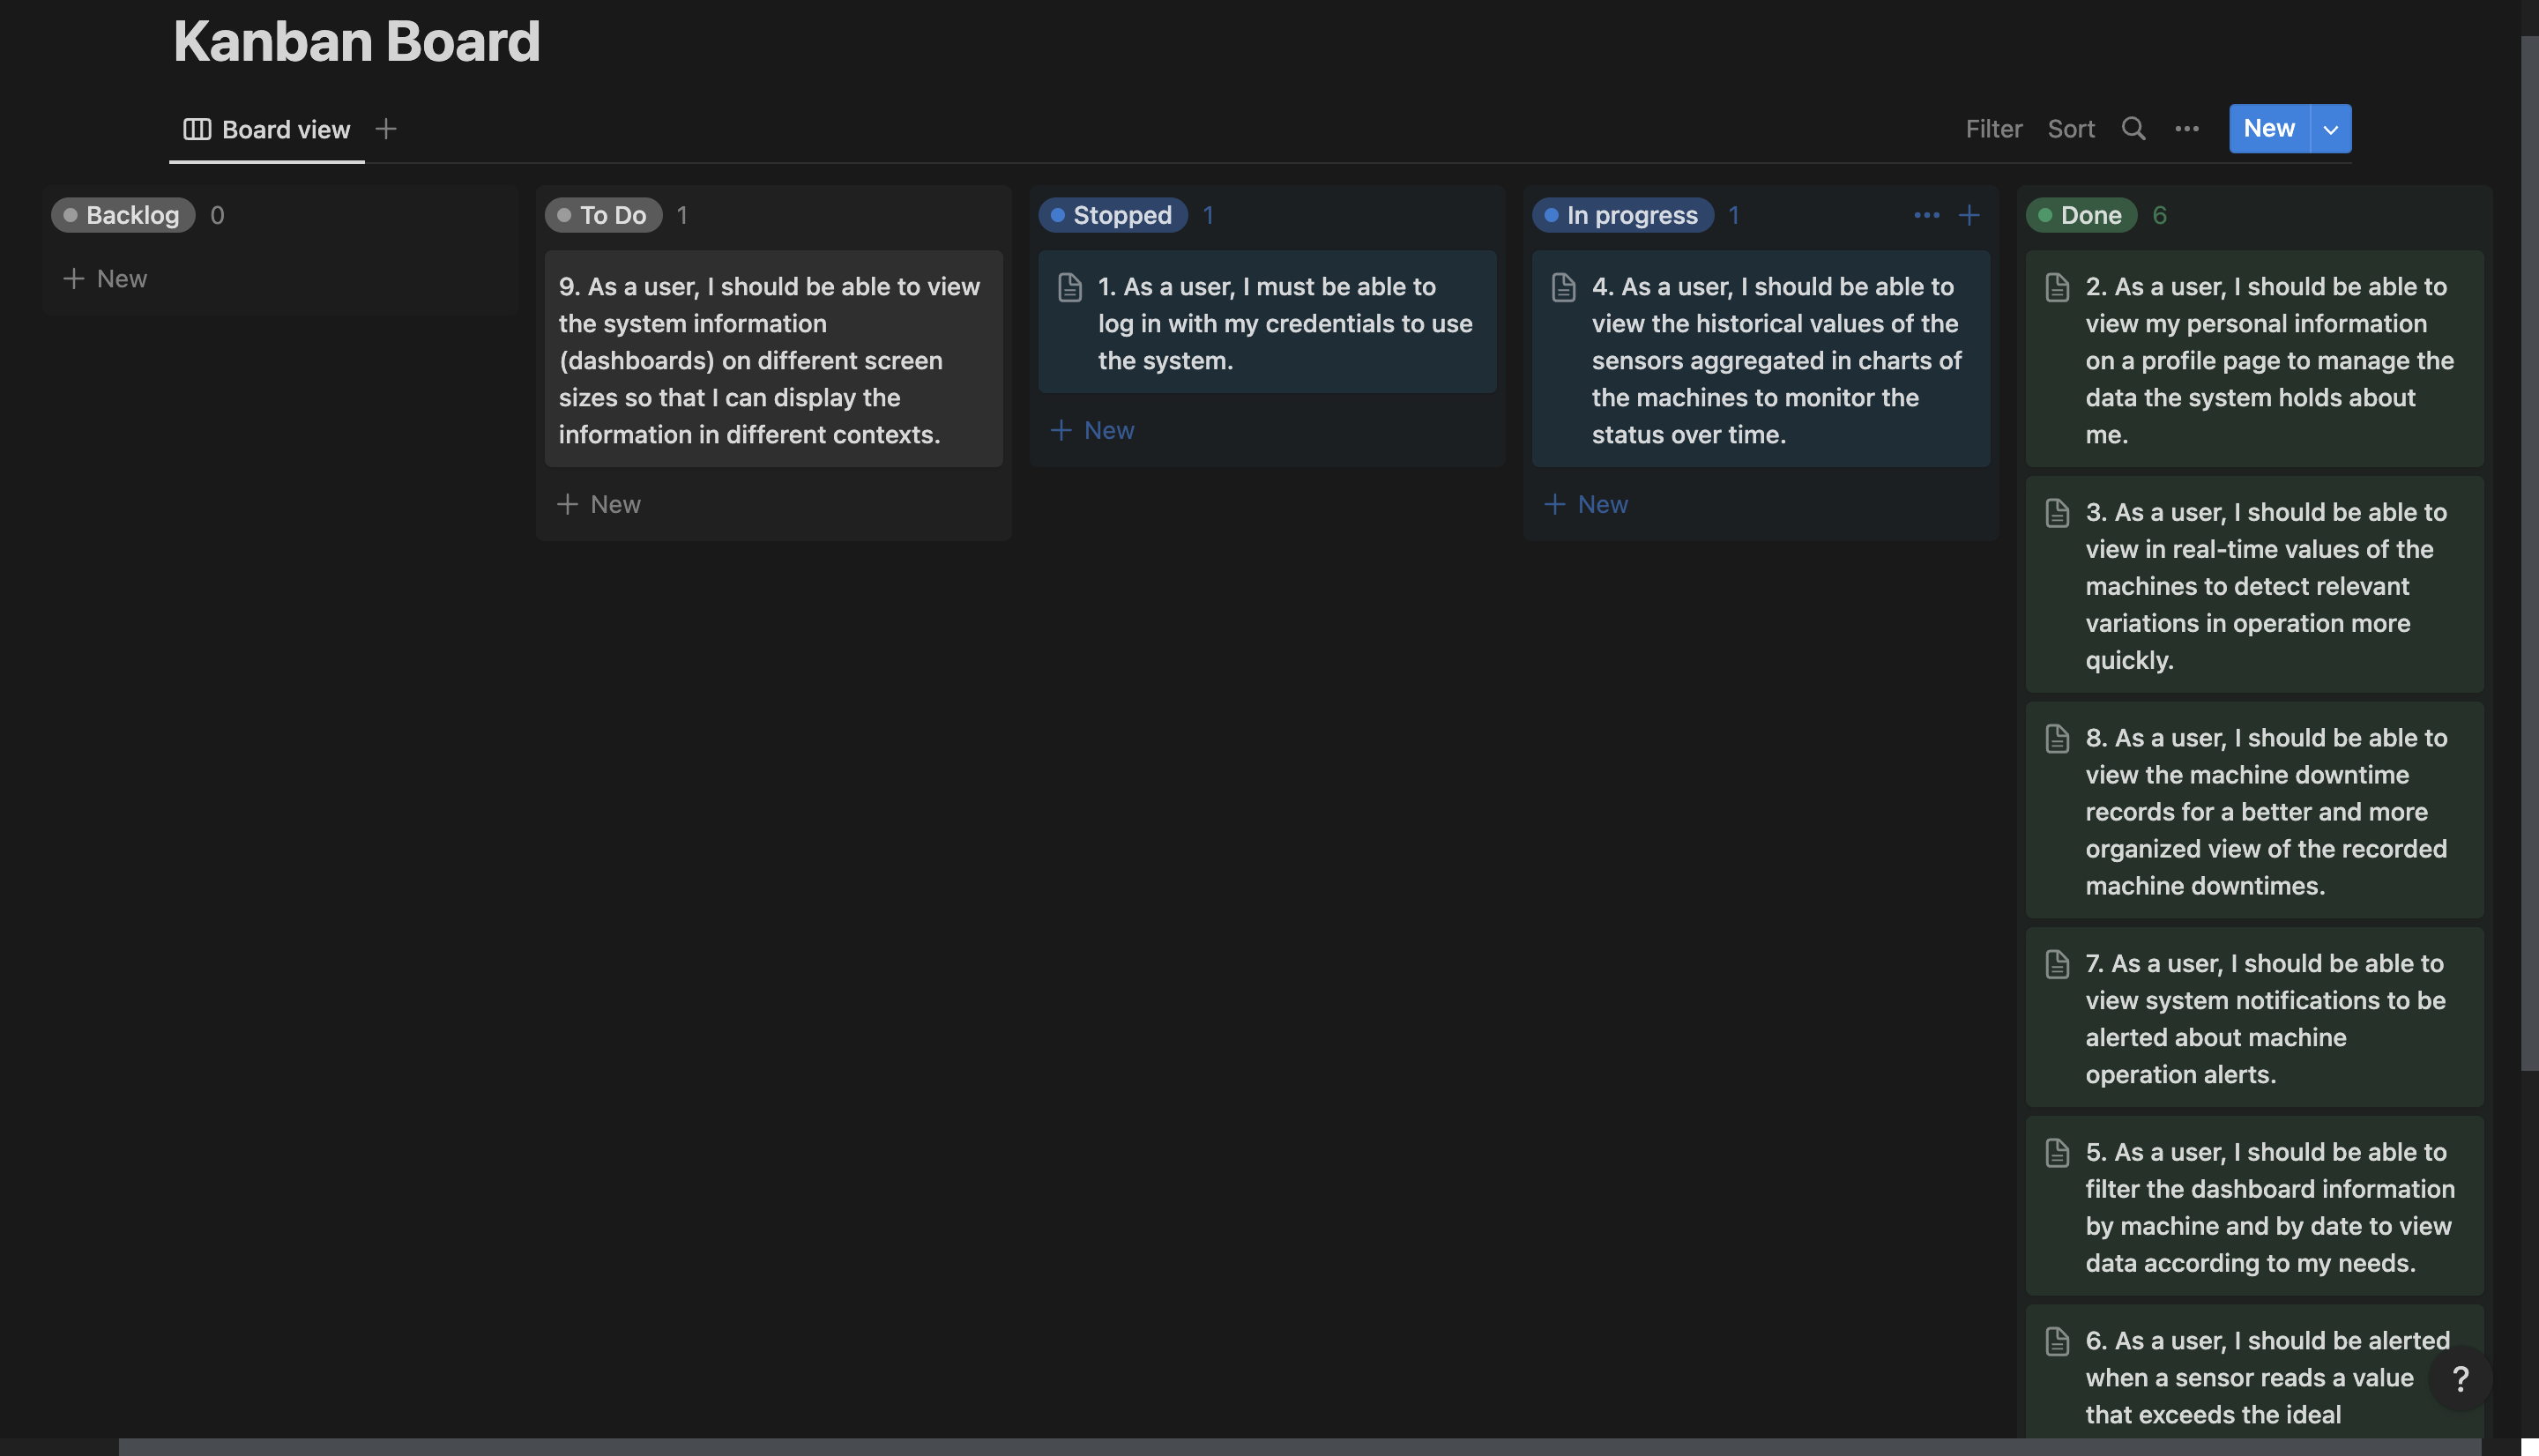
\includegraphics[scale=0.25]{images/kanban_board}
	\caption{Kanban board used to manage the tasks.}
	\label{fig:BoardKanban}
\end{figure}

In order to better define the implementation of each user story, each card on the Kanban board was detailed with a description that includes relevant business rules, references to functional and non-functional requirements, acceptance criteria, and sub-tasks. Before a user story can be moved to the "In Progress" column, it is essential that these fields are evaluated to ensure an understanding of the task scope. The acceptance criteria play an important role in verifying that a story meets all the established requirements before it is marked as completed.

To illustrate this process, user story number 1 is detailed.

\textbf{1. As a user, I must be able to log in with my credentials to use the system.}
\begin{itemize}
    \item \textbf{Description:} To ensure security and customization of the user experience, the system must have an authentication feature. The user must enter their credentials - usually a username or email address and a password - to access their account and the functionalities associated with it.
    \item \textbf{Relevant Business Rules:} 
        \begin{itemize}
            \item Users cannot access the system without authentication.
            \item Attempts to log into the system should be stored in the database.
            \item Passwords should be stored securely, using techniques such as hashing.
        \end{itemize}

    \item \textbf{Requirement References:}
        \begin{itemize}
            \item \textbf{Functional:} FR1
            \item \textbf{Non-Functional:} NFR2, NFR3, NFR6, NFR9 
        \end{itemize}

    \item \textbf{Acceptance Criteria:}
        \begin{itemize}
            \item The system must present a clear and intuitive login screen.
            \item After correctly entering the credentials, the user should be redirected to the system's home page (/dashboard).
            \item If the credentials are incorrect, the user should receive a clear error message.
        \end{itemize}

        \item \textbf{Sub-tasks:}
            \begin{itemize}
                \item Design the login screen interface.
                \item Build the login interface in the repository.
                \item Implement the user creation logic with password hash.
                \item Implement the authentication logic in the backend with \gls{JWT} Token.
                \item Test the security and effectiveness of the login functionality.
                \item Test if the \gls{API} is returning the \gls{HTTP} codes correctly.
            \end{itemize}

\end{itemize}



\subsection{Project Documentation}\label{sec:documentation}
The project documentation was created using the Notion tool. The choice for this project was based on the fact that Notion stands out for its flexibility, allowing an adaptable configuration of the text to meet various types of needs. The intuitive interface makes the insertion and updating of information a simple process, which can be executed as it is a platform accessible on the internet by any browser \cite{notionProjectManagement}.

In this way, the documentation was elaborated adopting a structured approach to ensure that all features and functionalities were properly cataloged. The basis of this documentation is a table, where each entry corresponds to a functionality or a specific part of the system, being named according to the name of the feature in question.

Each item in the table expands into an independent page, with descriptive details. This organization allows understanding in each aspect of the system, as it was being built as the system was developed, thus reflecting the most recent additions and changes.

To facilitate navigation and search for specific information, a tag column was incorporated into the table. These tags serve to categorize functionalities, and also an efficient search mechanism, allowing users to quickly identify the relevant aspects of the system.

In addition, the internal design of each page is based on the structure of markdown, explained in \cite{markdownguide}, to ensure that the content of the documentation is presented in a clear, structured, and aesthetically pleasing way, facilitating the understanding and absorption of information by the reader.

\subsection{Repository Configuration}
The platform chosen for managing the project's repositories was GitHub \cite{github}, one of the most renowned and widely adopted Git-based version control platforms currently available. The decision to use GitHub was based on several factors. Firstly, the platform offers an intuitive interface and a set of tools that facilitate tracking code progress, as well as collaboration among different team members. In addition, GitHub is recognized for its active community, which translates into resources, tutorials, and available support for resolving possible doubts and challenges. Finally, integration with other tools and platforms is possible if necessary, allowing for a continuous and optimized workflow. 

In this context, the repositories created for this project were \texttt{backend}, which stores the code related to the system's \gls{API} and Recive Data Module, another called \texttt{frontend}, which stores the code of the dashboard that is displayed on the web, another called \texttt{iot\_sensors\_data\_aggregation}, responsible for storing the code that performs the aggregation of the data received by the sensors, \texttt{SystemDataInitialization} which stores the code that initializes the database with the necessary data for the system to work, and finally \texttt{ServerConfiguration}, which stores the code that configures the web server that serves the dashboard. 

\subsection{Periodic meetings}
The development of the project was accompanied by meetings to ensure its alignment with the project objectives. Weekly meetings with the supervising professor were established, ensuring a constant review, time to ask questions, and to detail activities. These meetings provided continuous feedback, allowing for trajectory correction and focus on the desired progress for the project. In parallel, monthly meetings were conducted with the interested company, to present what was being built, gather feedback, guidance on desired features, and also to better understand how the company operates and its needs.

These meetings played a fundamental role in integrating academic research and the practical needs of the industry, ensuring that the developed solutions remained relevant and applicable to the business context. This supervision system was crucial in keeping the project on track, balancing academic needs with industrial applicability within the company's context.

\section[Tecnologias]{Technologies}
The selection of technologies was carried out to meet specific requirements of scalability and long-term sustainability. Given that the system is primarily aimed at data storage and management, its use as a reference for future projects with similar characteristics was anticipated, therefore, the emphasis was placed on modern technologies, widely recognized and with robust support in the development community.

In this context, MongoDB was chosen as our non-relational database solution, due to its flexibility and performance. Python was adopted as the language for the backend, due to its versatility and extensive library. The FastAPI framework, in turn, was employed for the development of the \gls{API}, thanks to its efficiency and ease of integration. In the frontend scope, the JavaScript language was complemented by the NextJs framework, recognized for its optimization and advanced features. To ensure a fluid and modular integration of the system components, Docker containers were used, while efficient web server management was ensured by NGINX.

\subsection{MongoDB}

When selecting a database platform, MongoDB \cite{mongodbDocs} was chosen, a non-relational database system designed to flexibly adapt to changes in the format of the data that is stored. MongoDB provides ease in manipulating the data lake in various contexts. Its meticulously structured documentation, coupled with a vast range of content available online, proved to be invaluable for knowledge acquisition.

Distinctively, MongoDB presents advantages such as the ability to support distributed and parallel queries, optimizing the processing of intricate requests in scenarios with significant data density. Additionally, its compatibility with a wide variety of data analysis tools sets a promising precedent for future evolutions of the project.

\subsection{Python}
In the development of the backend, the Python language \cite{pythonOfficialDocs} was chosen, widely recognized for its versatility, readability, and adaptability in various application contexts. Python, being one of the most popular and widely accepted languages in the academic and industrial world, presents a vast standard library and robust community support. The rich range of educational materials, which spans from detailed tutorials to extensive discussion forums, was essential for learning.

Python's intuitive syntax favors rapid prototyping and development, while the wide range of available frameworks and libraries enhances its application in various aspects, from data analysis to web development. These intrinsic characteristics, combined with the language's flexibility and efficiency, consolidate the decision to adopt Python as the central language for the backend in this master's project.

\subsection{FastAPI}
In the backend implementation, the Python language was used in conjunction with the FastAPI framework \cite{fastapiDocs}. The motivation behind this choice came from FastAPI's efficiency and high performance. An important feature is its integration with the \gls{ASGI} library. This library significantly refines request management by providing asynchronous processing, thus ensuring faster and more accurate responses.

FastAPI's comprehensive documentation is also a factor that contributes to its choice. For developers, especially those in the field of software engineering, well-structured documentation serves as an important learning resource. It not only accelerates the learning curve but also assists when facing potential problems and doubts during the development phase.

Another significant aspect of FastAPI is its support for data validation with the Pydantic library. Through Pydantic, it is possible to validate data types and structures, ensuring that the received data aligns with the expected formats. This functionality not only reinforces the robustness of the application but also minimizes runtime errors originating from unexpected data inputs.

In addition, FastAPI facilitates API documentation through its integration with Swagger UI \cite{swaggerui2023}. This means that as developers design and implement API endpoints, a documentation interface is automatically generated. This serves as a great advantage for developers and end users, enabling real-time testing, understanding, and interaction with the API, thus improving the overall development and usage experience.

\subsection{NextJs}
For the frontend architecture, the choice was made to use Next.js \cite{nextjsDocs}, a framework that significantly enhances the interaction with the JavaScript React library \cite{reactDocs}, as emphasized in the official React documentation itself. Community support is one of its main features, being widely complemented by a range of educational materials available on the internet - from tutorials to blog articles and instructional videos - which contributed essentially to the learning process.

In the scope of this project, alongside Next.js, TypeScript \cite{typescriptLang} was incorporated, which, due to its static typing nature, provides a more intuitive code maintenance, increasing its readability, simplifying its understanding and management.

The coherence between Next.js and TypeScript establishes a highly effective development environment. While Next.js promotes a more fluid and high-performance development experience, TypeScript strengthens security and productivity, thanks to its rigorous typing. These factors justify the choice of the combination of Next.js and TypeScript for the realization of this project.

In addition to Next.js and TypeScript, Material UI 5 \cite{muiDocs} was integrated into the project as a user interface design library. This set of React components, based on Google's Material Design standard \cite{m3Docs}, offers a wide range of already stylized and easy-to-implement interface elements. Besides saving time in developing components from scratch, the library provides a cohesive and modern user experience. The use of Material UI 5 also contributes to the standardization of design throughout the project, ensuring a more intuitive and pleasant user experience. Therefore, the addition of this feature effectively complements the already robust capabilities offered by the combination of Next.js and TypeScript, making the development environment even richer and more productive.

\subsection{Docker}
For the orchestration and management of the development and production environment, Docker \cite{dockerDocs} was adopted as the containerization tool. Docker, widely recognized in the software development universe, allows encapsulating applications and their dependencies in containers, ensuring uniformity, reproducibility, and isolation among environments \cite{dockerOverview}. This approach significantly simplifies integration, testing, and deployment processes, as containers can be transparently moved between different environments and platforms.

The extensive documentation available, along with an active community, provided a clear understanding and facilitated the adoption of this technology. In addition, the flexibility and efficiency provided by Docker, by minimizing dependency conflicts and ensuring that the application works consistently in various contexts, were decisive factors for its choice in this project.

\subsection{NGINX}
For the part of managing web requests, NGINX \cite{nginxDocs} was adopted as the web server. NGINX is recognized for its high performance, reliability, and flexibility, making it a suitable choice in production environments that demand low latency, efficient handling of a large number of simultaneous connections, and the ability to serve static content extremely quickly. These characteristics make it particularly suitable for systems aiming for scalability and robustness.

The extensive documentation and the vast community resources were essential to deepen the understanding and apply best practices in the project context. Considering the need for a consistent and optimized delivery of content to the end user, as well as a secure and effective proxy configuration, NGINX proved to be the preeminent choice for this master's dissertation.






